%%%%%%%%%%%%%%%%%%%%%%%%%%%%%%%%%%%%%%%%%
% Journal Article
% LaTeX Template
% Version 1.4 (15/5/16)
%
% This template has been downloaded from:
% http://www.LaTeXTemplates.com
%
% Original author:
% Frits Wenneker (http://www.howtotex.com) with extensive modifications by
% Vel (vel@LaTeXTemplates.com)
%
% License:
% CC BY-NC-SA 3.0 (http://creativecommons.org/licenses/by-nc-sa/3.0/)
%
%%%%%%%%%%%%%%%%%%%%%%%%%%%%%%%%%%%%%%%%%

%----------------------------------------------------------------------------------------
%	PACKAGES AND OTHER DOCUMENT CONFIGURATIONS
%----------------------------------------------------------------------------------------

\documentclass[twoside,twocolumn]{article}


\usepackage{blindtext} % Package to generate dummy text throughout this template 
\usepackage{graphicx}
\usepackage{hyperref}

\graphicspath{ {images/} }

\usepackage[sc]{mathpazo} % Use the Palatino font
\usepackage[T1]{fontenc} % Use 8-bit encoding that has 256 glyphs
\linespread{1.05} % Line spacing - Palatino needs more space between lines
\usepackage{microtype} % Slightly tweak font spacing for aesthetics

\usepackage[english]{babel} % Language hyphenation and typographical rules

\usepackage[hmarginratio=1:1,top=32mm,columnsep=20pt]{geometry} % Document margins
\usepackage[hang, small,labelfont=bf,up,textfont=it,up]{caption} % Custom captions under/above floats in tables or figures
\usepackage{booktabs} % Horizontal rules in tables

\usepackage{lettrine} % The lettrine is the first enlarged letter at the beginning of the text

\usepackage{enumitem} % Customized lists
\setlist[itemize]{noitemsep} % Make itemize lists more compact

\usepackage{abstract} % Allows abstract customization
\renewcommand{\abstractnamefont}{\normalfont\bfseries} % Set the "Abstract" text to bold
\renewcommand{\abstracttextfont}{\normalfont\small\itshape} % Set the abstract itself to small italic text

\usepackage{titlesec} % Allows customization of titles
\renewcommand\thesection{\Roman{section}} % Roman numerals for the sections
\renewcommand\thesubsection{\roman{subsection}} % roman numerals for subsections
\titleformat{\section}[block]{\large\scshape\centering}{\thesection.}{1em}{} % Change the look of the section titles
\titleformat{\subsection}[block]{\large}{\thesubsection.}{1em}{} % Change the look of the section titles

\usepackage{fancyhdr} % Headers and footers
\pagestyle{fancy} % All pages have headers and footers
\fancyhead{} % Blank out the default header
\fancyfoot{} % Blank out the default footer
\fancyhead[C]{Predictive Analysis in Industrial Safety Applications $\bullet$ MSA Safety Hackathon $\bullet$ April 2018} % Custom header text
\fancyfoot[RO,LE]{\thepage} % Custom footer text

\usepackage{titling} % Customizing the title section

\usepackage{hyperref} % For hyperlinks in the PDF

%----------------------------------------------------------------------------------------
%	TITLE SECTION
%----------------------------------------------------------------------------------------

\setlength{\droptitle}{-4\baselineskip} % Move the title up

\pretitle{\begin{center}\Huge\bfseries} % Article title formatting
\posttitle{\end{center}} % Article title closing formatting
\title{Predictive Analysis in Industrial Safety Applications} % Article title
\author{%
\textsc{Steven Shan, Serano Tannason, Brandon Pek} \\[1ex] % Your name
\normalsize Carnegie Mellon University \\ % Your institution
\normalsize \href{mailto:slshan@andrew.cmu.edu}{slshan@andrew.cmu.edu}
$\bullet$
\normalsize \href{mailto:stng@andrew.cmu.edu}{stng@andrew.cmu.edu}
$\bullet$
\normalsize \href{mailto:bpek@andrew.cmu.edu}{bpek@andrew.cmu.edu}
%\and % Uncomment if 2 authors are required, duplicate these 4 lines if more
%\textsc{Jane Smith}\thanks{Corresponding author} \\[1ex] % Second author's name
%\normalsize University of Utah \\ % Second author's institution
%\normalsize \href{mailto:jane@smith.com}{jane@smith.com} % Second author's email address
}
\date{\today} % Leave empty to omit a date
\renewcommand{\maketitlehookd}{%
\begin{abstract}
\noindent Data analytics have improved organizations' understanding of ways to mitigate danger in the workplace. Oil and mine plants are one application that stood out to us, in particular, due to their high risks as well as the potential to apply results from data analysis to constructing a safer environment for workers to work in. We utilized the data that were provided to us by the MSA to analyze possible trends in sensor readings and alarm activities. Based on our parsed data, we were able to drew conclusions from the charts produced. We include suggestions for improvements, especially in the data collection phase. We also propose an interactive web application that could be used to improve worker engagement and ultimately improve safety in high-risk environment.
\end{abstract}
}

%----------------------------------------------------------------------------------------

\begin{document}

% Print the title
\maketitle

%----------------------------------------------------------------------------------------
%	ARTICLE CONTENTS
%----------------------------------------------------------------------------------------

\section{Introduction}

This is our submission for the 2018 MSA Safety Hackathon on methods for improving worker safety at gas production facilities based on analysis of sensor data and alarms triggered during a four month period. It is for the \texttt{Predictive Analysis} category of the hackathon although we include some business like methodology with the proposal at the end. We begin with a quick suggestion based on our experience working with the data using methodology described in the following methods section. All of the data we worked with is available in our Git repository and can be extracted using the provided \texttt{setup.py} file. We then list some suggestions for organizing the data and our analysis of the data. Finally, we have a proposal for a website portal for workers to view incident history as well as safety guidelines.

%------------------------------------------------

\section{Suggestions}

The way the data is currently stored, if sensor readings in parts per million (PPM) reaches a certain threshold, they will trigger an alarm. We believe that standardizing thresholds on a scale of 0 to 10, workers will be able to be better understand the severity of the situation. For example, as it currently is hydrogen sulfide ($H_2 S$) has a low threshold of 10 while methane has a low threshold of $0.5$. If a worker were to briefly look at the readings, and see a reading of $1.0$ for both, they might think they are perfectly within safe thresholds because $H_2 S$ has a threshold a factor of 10 greater. This could pose a major safety hazard because methane actually has a much lower threshold. By standardizing a scale, workers could better judge the safety of the environment with the gas readings. In addition, a scaling factor could be includied in the data to convert from the scale to each threshold to PPM so that no data is lost in this process.\\\\
We suggest scaling each reading for parts per million to a 0 to 10 scale where a 0 would be safe, 5 would be lower exposure, and 10 would be high exposure. This removes the human error element when workers have to memorize safe PPM thresholds for each gas reading since a rating from 5 to 10 would represent a dangerous environment regardless of gas type.\\\\
We also include a proposal for a website service at the end of this paper.

%------------------------------------------------

\section{Methods}

Our method involves two phases: data extraction and data analysis.\\\\
For data extraction, we began by processing the provided periodic and session data files. Our processed data can be retrieved by running
\begin{verbatim}
python setup.py all
\end{verbatim}\footnote{Requires Git LFS and Python 2.7}
in the root directory of the repository. This will uncompress the provided data as well as the parsed JSON files and Python pickles.\\\\
We repurposed an HTML parser to read convert the provided XML data files into a tree structure where each nodes represents an XML tag. This structure was then converted into a Python dictionary object. A major obstacle in this step was there was no intuitive way to write duplicate keys in the dictionary since many XML tags such as \texttt{Sensor} or \texttt{Alarm} had duplicates under the same parent tag. We approached this by taking the duplicates and combining them in a list under a single key.\\\\
The parser was run on each of the periodic and session data files and the results were combined into lists and exported to JSON as \texttt{data/periodic.json} and \texttt{data/session.json}.\\\\
We then converted these huge JSON files into Comma-Separated Values (CSV) format, which is compatible with Microsoft Excel. To do so, we traversed through the chain of nested dictionaries and extracted the relevant fields such as \texttt{Temperature}, \texttt{MineSite}, and \texttt{Peak} for addition into the CSV files.\\\\
Using Excel and our CSV files, we were able to produce the scatter-plot and line charts attached in this document. In our analysis, we decided to emphasize the \texttt{average} and \texttt{peak} gas sensor readings fields in both Session Alarm and Periodic Details files. We plotted these two fields against the date and time that these readings were taken, and further categorized the plots for Periodic Details data into the three sites we found in the data files. Note that there were no readings from Site 4.

%------------------------------------------------

\section{Suggestions for Data Organization}

While working with the provided data, we noticed several ways the organization and storage of the data could be improved.
\begin{enumerate}[leftmargin=*]
\item In the \texttt{Session Alarm Details 108} XML file there appears to be a millenial bug or error where the time was set to 0 because one of the timestamps shows \texttt{1/1/0001 12:00:00 AM}. While we don't know the purpose of the tag, such an error could cause errors in reporting the alarm that may pose a safety threat.
\item Although this may be the result of redacted data, we found it difficult to find a link between the periodic data files and session data files. We believe that each session data file represents a discrete time that an alarm was triggered and contains a short segment of sensor readings before and after the alarm. However, without a way of finding the corresponding periodic data file, we felt limited in the amount of information about sensor readings leading up to the time the alarm was triggered.
\item We noticed that in the \texttt{Sensors} tag in session data files, there were several alarms listed such as \texttt{ExposureLowAlarm}, \texttt{ExposureHighAlarm}, and \texttt{TWA} (Time Weighted Average) along with their associated thresholds, but when we looked at the actual \texttt{AlarmType} for the reports, there were other alarms such as \texttt{ExposurePeakAlarm}. This additional alarm could be included in the \texttt{Sensors} tag or in additional documentation.
\item We believe that JSON would be a more appropriate format for storage of the data files instead of XML. While XML has support for schemas and namespaces, the files do  not make use of these features which are the main benefit of using XML over JSON. In general, JSON would make it easier to parse the data especially in a web environment since Javascript has native support for JSON parsing.
\end{enumerate}

%------------------------------------------------

\section{Results}

\begin{figure*}
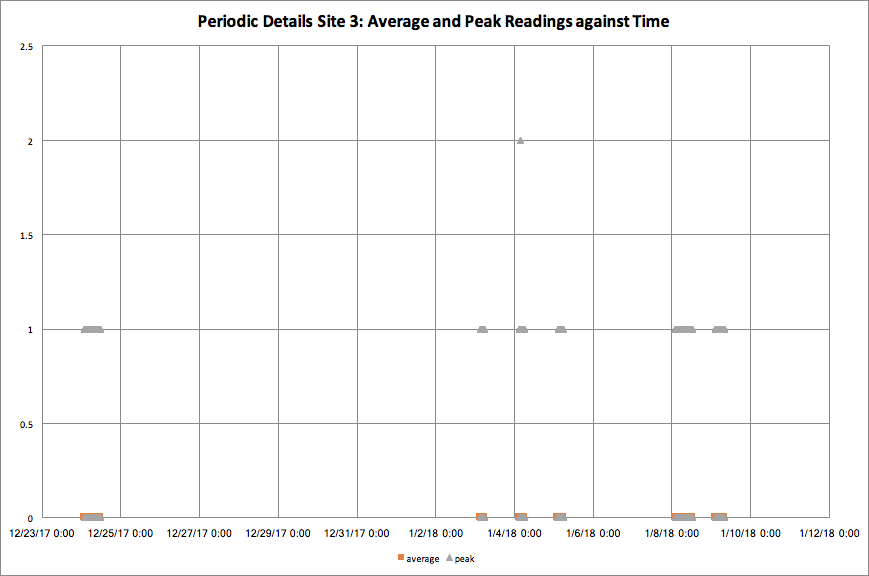
\includegraphics[width=15.1cm]{images/image5.png}
\caption{Average and Peak Readings from Periodic Details (Dec 2017 - Jan 2018)}
\end{figure*}
\begin{figure*}
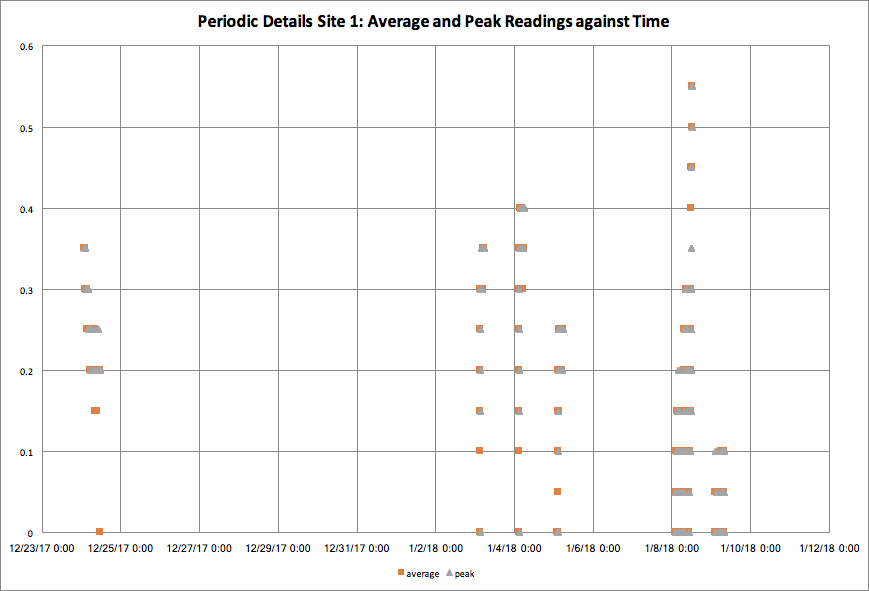
\includegraphics[width=15.1cm]{images/image4.png}
\caption{Average and Peak Readings for Site 1 from Periodic Details  (Dec 2017 - Jan 2018)}
\end{figure*}
\begin{figure*}
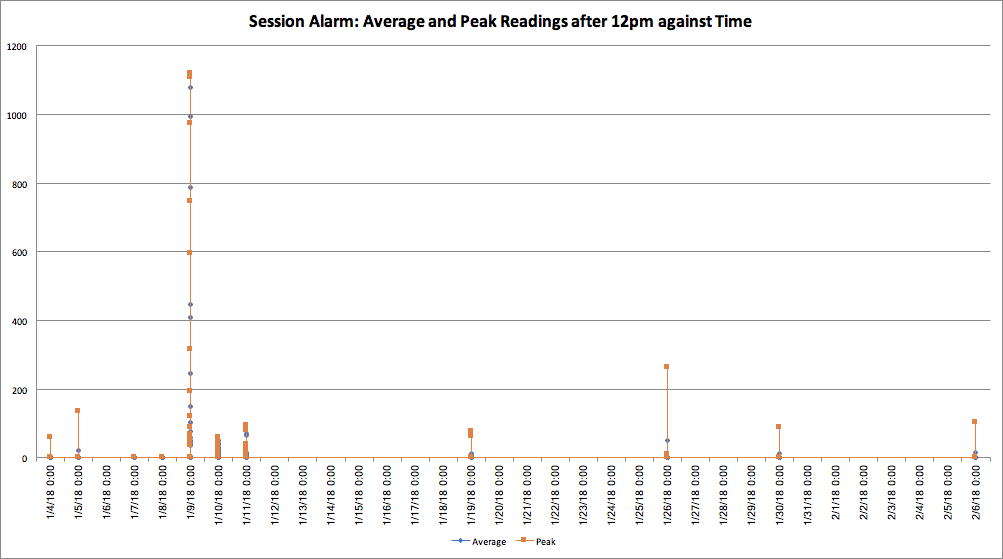
\includegraphics[width=15.1cm]{images/image2.png}
\caption{Average and Peak Readings for Site 3 from Periodic Details (Dec 2017 - Jan 2018)}
\end{figure*}
\begin{figure*}
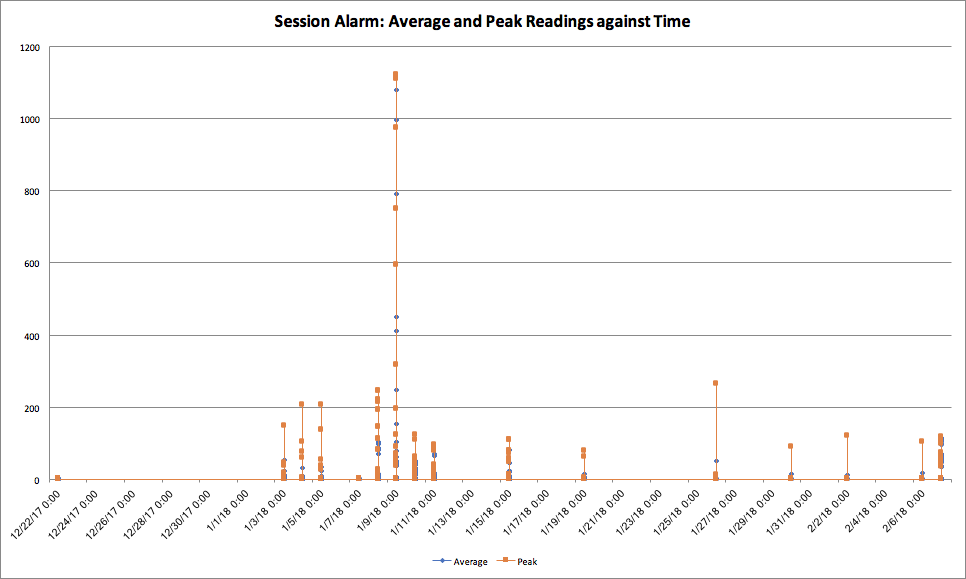
\includegraphics[width=15.1cm]{images/image1.png}
\caption{Average and Peak Readings from Session Alarm Reports (Dec 2017 - Feb 2018)}
\end{figure*}
\begin{figure*}
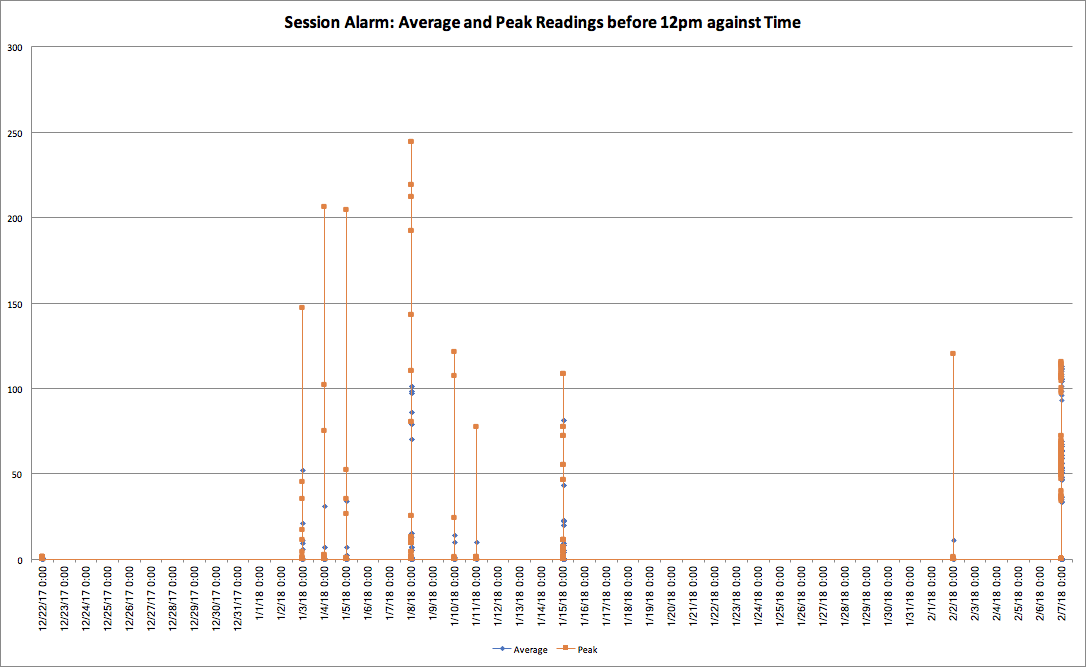
\includegraphics[width=15.1cm]{images/image6.png}
\caption{Average and Peak Readings from Session Reports before 12pm  (Dec 2017 - Feb 2018) 9 spikes were observed.}
\end{figure*}
\begin{figure*}
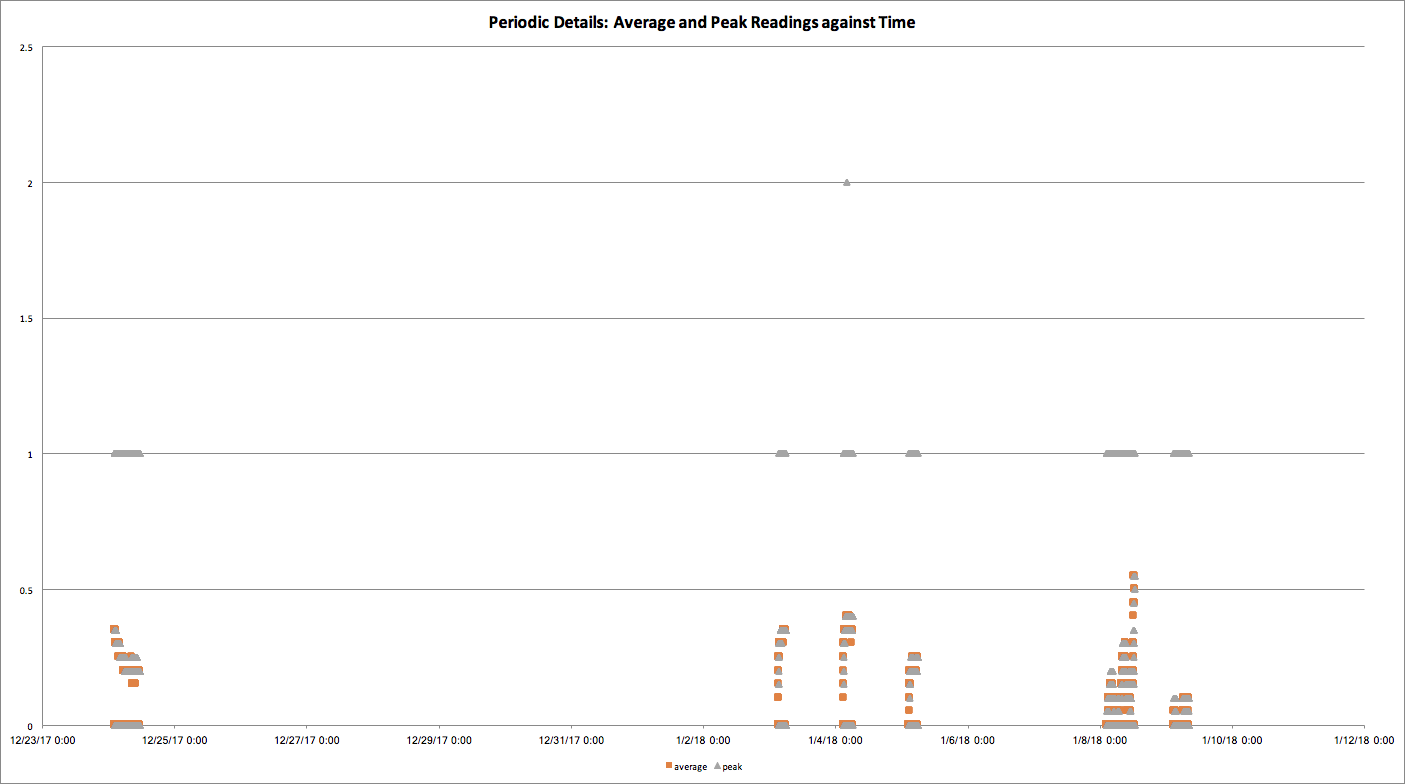
\includegraphics[width=15.1cm]{images/image3.png}
\caption{Average and Peak Readings from Session Reports after 12pm (Dec 2017 - Feb 2018) 9 spikes were observed.}
\end{figure*}
We initially hypothesized that some of the attributes available in the data provided could have been a contributing factor to the frequency of alarm triggers and gas sensor readings. We considered the possibility of there being a correlation between time of the day, temperature, or week periods and the readings obtained. We hereby report that with the data provided, we were not able to find any certain correlation between these values. Our findings might have been inconclusive due to the data only spanning three months from December 2017 to February 2018, and that sensor readings were taken infrequently only on some days of the month. However, this might also suggest that the unreported days of the month were accident-free, which may not be a negative sign.\\\\
Furthermore, we observe in Figure 1 while analyzing average and peak readings over time from ``Periodic Details'' that huge spikes in gas readings occur very spontaneously and infrequently.\\\\
In figures 2 and 3, we split the data plots based on sites 2 and 3 and noted in figure 1b that site 2 seemed to have more occurences of sustained gas leaks. On the other hand, site 3 had a few peaks of gas leaks but was on average relatively mild.\\\\
Figures 4 through c record our findings from the Session Alarm Reports. One interesting note is that some outliers, such as the reading over 1000 seem to suggest that the gases being measured are different gases and are measured using different scales. However, as some of the gas names were redacted, we were unable to make that distinction. Nevertheless, the readings that are scattered closely during the January 9 period seem alarmingly high and could warrant some inspection on the circumstances leading up to that peak gas leakage period.\\\\
In figures 5 and 6, we attempted to see if there was a relationship between gas leak and time of the day. Figure 5 records the gas measurements taken before 12pm and figure 6 records gas measurements taken after 12pm. Due to the limited span of data sampling, we observed that there were 9 significant gas spikes for each time period, and hence could not reach a conclusive relationship between time of day and gas leak. Perhaps a quantitative method to discover this relationship, if it might interest MSC, would be to fix a sensor at the site and take regular sensor readings over fixed time intervals.

%------------------------------------------------

\section{Proposal}

\subsection{Overview}

In this project, we decided to focus on data extraction and analytics but have mapped out the concept of building a portal for workers. Whereas the data provided to us were entirely based on sensor readings, we believe that allowing workers to input their experience and feedback is of tremendous value to improving the safety system implemented. Moreover, we believe that worker engagement offered by this portal is critical to encourage safe practices in the field.\\\\ 
Having recognized that the key to safety lies in constant and timely reinforcement of precautionary measures that are tangible and easy to act on, we envision a web portal that resembles a daily log, except more intelligent.

\subsection{Proposed Safety Website Portal}

The web portal will be used by workers or supervisors at the start of every shift, and will take in four data fields: (1) the nature of activity, (2) the location of work site, (3) safety equipment being used. If an accident occurs during the work shift, the log can be updated at the end of the shift with the fourth data field (4) accident details.\\\\
The backend of the web portal will first be initialized with statistics of past gas leaks and/or safety breaches. Our risk-assessment matrix will take in four fields: (1) nature of activity, (2) location of work site, (3) safety equipment being used and (4) record of past accidents to generate a predicted risk score from 0 to 1. We envision that the record of past accidents can be analyzed using statistical regression or neural networks, if data fields are sufficient, to generate the risk score. Each time our web portal is used, our algorithm has access to more data and can better generate risk scores.\\\\
With the back-end having generated a predicted risk score, the worker or supervisor will now be redirected to the results page that will display four fields: (1) risk score, (2) details of last known incident at the site of interest, (3) recommended safety products from MSA if the worker is deemed to have insufficient safety equipment and (4) recommended safety drills or a customized message from higher superiors on special instructions to note on this particular site/nature of activity.\\\\
There are many unpredictable risk factors in the industrial field of gas and oil plants or mines that can escape human calculations, however, there are also risk factors that can be mitigated with human intervention, hence the importance of reinforcing safety drills and familiarity with precautionary measures right before each work shift. This is a practice adopted on airlines with their repetitive safety demonstrations before each flight takes off, or with militaries conducting ``Just In Time'' drills before handling live firearms. Therefore our proposed web app aims to ensure every worker goes into his/her shift with refreshed familiarity of precautionary measures to adopt in hostile situations, as well as a brief understanding of risk score and history of this worksite.\\\\
These features complement the gas detection hardware in place but will still rely on readings from gas detection to develop a smarter algorithm with better predicting accuracy.\\\\
In addition to addressing the grassroots through reinforcement learning, a safety culture has to be propagated by clear policy decisions by senior management. This can also be addressed by our web app which provides a much clearer data visualization of the implications of gas leaks. We mean clearer data visualization in terms of the inclusion of helpful data fields like number of accident-free man hours, frequency of accidents within the sample space and ultimately the useful quantitative risk score. A quantitative-based approach could lead to further findings with regards to relationships between accident occurrence with time of the day, temperature, and what measures could be done to reduce the risk score.

%----------------------------------------------------------------------------------------
%	REFERENCE LIST
%----------------------------------------------------------------------------------------

\begin{thebibliography}{99} % Bibliography - this is intentionally simple in this template

\bibitem[Wachter and Yorio]{}
Jan K. Wachter and Patrick L. Yorio. Indiana University of Pennsylvania, Safety Sciences Department, Johnson Hall Room 137, 1010 Oakland Avenue, 15705-1063, United States
\newblock \url{https://www.sciencedirect.com/science/article/pii/S0001457513002972}
  study.
 
\end{thebibliography}

%----------------------------------------------------------------------------------------

\end{document}
